%atmospheric O3 with budget, lifetime, stratospheric & tropospheric ozone
Ozone (\ce{O3}) is an atmospheric constituent gas found in the stratosphere and troposphere, however its atmospheric effects are very different in these distinct regions.
About 90\% of the atmospheric ozone is present in the stratosphere, with a peak mixing ratio of about 12 ppm \citep{Seinfeld:2006}.
Stratospheric ozone absorbs the sun's ultraviolet radiation in the wavelength region 280 - 315 nm, this is extremely important as excess UV radiation can cause skin cancer, cataracts and a suppressed immune system in humans and can also damage plant, single-cell organisms and aquatic ecosystems \citep{WMO:2010}. 

In contrast, tropospheric ozone that is found close to the surface is both a pollutant and a greenhouse gas. 
Increased levels of tropospheric ozone are harmful to humans, plants and other living systems, as high ozone exposure can lead to pulmonary problems in humans and can decrease both crop yields and forest growth \citep{WMO:2010}. 

Globally, tropospheric ozone is formed mainly via chemical production and downward transport from the stratosphere into the troposphere, called the Stratosphere-Troposphere Exchange (STE) may also play a role. 
The STE is driven by the Brewer-Dobson circulation \citep{Brewer:1949, Dobson:1956}.  
This is a relatively slow circulation (over a timescale of weeks to months) and is due to planetary wave disturbances in the troposphere \citep{Haynes:1991}.
The circulation causes air to move downward from the stratosphere into the troposphere at the mid at high latitudes and is balanced by upward exchange at the tropics. 
The STE also has a seasonal variability where the maximum transport occurs during spring \citep{Appenzeller:1996}, due to the increase in altitude of the tropopause - the boundary level between the troposphere and the stratosphere - which moves stratospheric air into the troposphere. 

A spring-time peak in \ce{O3} concentration is common in many areas, especially in the midlatitude Northern Hemisphere, and it was originally thought that the STE was mainly responsible. 
However, it is only very rarely that \ce{O3} originating via STE can influence tropospheric \ce{O3} levels \citep{Lelieveld:2000}. 
It was later realised that this spring maximum is due to the photochemical reactions occuring in the Northern Hemisphere spring after the buildup of reservoir species over winter \citep{Penkett:1986} that are then oxidised photochemically, the increase in these reactions is due to the increase in temperature, moisture and sunlight.
Hence, photochemical reactions are the major source of surface tropospheric ozone \citep{Lelieveld:2000} and since \ce{O3} is produced in this way it is termed a secondary pollutant.

%metereology impacts 
Tropospheric \ce{O3} is not only impacted by emission levels, it is also affected by meteorological variables such as temperature, number of hours of sunshine and wind as these impact transport, dry and wet deposition rates and also chemical reaction rates \citep{Hess:2009}.
Meteorology influences both regional and global \ce{O3} \citep{Hess:2009}, climate patterns such as El Ni\~{n}o are also known to impact \ce{O3} levels in certain areas \citep{Sudo:2001}. 

The effect of meteorology is an aspect of atmospheric chemical transport modelling that needs to be taken into account. 
However it is also frequently the major source of uncertainty for the calculated \ce{O3} concentrations. 
Wind speeds in particular may lead to under- or over-predicated values of \ce{O3} concentrations \citep{Sillman:1999}. 

In general, there is great effort to reduce anthropogenic emissions that impact air quality and human health. 
For example, the EPA in the US and European Union all have regulations related to air quality with a set exceedance limit for \ce{O3} concentrations. 
Many cities in the US, especially in the northeast and southern California, have reduced the emissions of \ce{O3} precursors - mainly volatile organic compounds (VOC) emissions - due to repeated exceedances \citep{Fiore:1998}. 
These VOC emission reductions have proven successful as the amount of \ce{O3} in these metropolitan areas has been decreased despite nitrogen oxide levels, which also impact \ce{O3} levels, being almost constant \citep{Fiore:1998, Lin:2001}.

Modelling of \ce{O3} has greatly influenced the understanding of complexity of atmospheric chemistry, for example the non-linear relationship of \ce{O3} production on the VOC and nitrogen oxides concentrations. 
This in turn has led to a better understanding on how to reduce the \ce{O3} levels for better air quality. 
The need for more realistic and effective air quality standards in turn also drives the model development and deeper understanding of atmospheric chemistry. 
Providing detailed information of which VOCs can produce the most \ce{O3} is of greater benefit for regulation purposes rather than lumping all VOCs under one common regulation. 
Moreover, this can give indication on possibly replacement substances in order to improve air quality.

\section{Tropospheric Chemistry} \label{s:atmo_chem}

\subsection{Ozone Chemistry}
%O3 chemical sources & sinks, linking VOCs.
Troposperic ozone is principally formed by the photolysis of nitrogen dioxide (\ce{NO2}), which produces nitrogen oxide (NO) and a ground state oxygen atom (\ce{O(^3P)}), this then reacts with molecular oxygen (\ce{O2}) to form \ce{O3}. 
Ozone reacts rapidly with NO to return \ce{NO2} and \ce{O2}, this is represented by the following reaction cycle.
\begin{reactionlist}
    \reactionitem{\ce{NO2 + $h\upsilon$}}{NO + \ce{O(^3P)}}{new}{r:NO2photo}
    \reactionitem[M]{\ce{O(^3P) + O2}}{\ce{O3}}{new}{r:O3form}
    \reactionitem{\ce{NO + O3}}{\ce{NO2 + O2}}{new}{r:NO+O3}
\end{reactionlist}
These reactions do not produce net \ce{O3}, due to a photoequilibrium between NO, \ce{NO2} and \ce{O3} \citep{Atkinson:2000}. 
Adding VOCs of both biogenic and anthropogenic origin, such as methane (\ce{CH4}), and other gas-phase compounds, such as carbon monoxide (CO) - to the mix, results in net \ce{O3} production. 
The oxidation mechanism of CO, taking into account reactions that give maximum \ce{O3} yield, is
\begin{reactionlist}
    \reactionitem[\ce{O2}]{\ce{CO + OH}}{\ce{CO2 + HO2}}{new}{r:CO+OH}
    \reactionitem{\ce{HO2 + NO}}{\ce{NO2 + OH}}{new}{r:HO2+NO}
    \reactionitem{\ce{NO2 + $h\upsilon$}}{\ce{NO + O(^3P)}}{old}{r:NO2photo}
    \hline
    \reactionitem{Net: \ce{CO + 2O2 + $h\upsilon$}}{\ce{CO2 + O3}}{new}{r:netCO}
\end{reactionlist}
whilst the oxidation mechanism of \ce{CH4} with maximum \ce{O3} yield is
\begin{reactionlist}
    \reactionitem[\ce{O2}]{\ce{CH4 + OH}}{\ce{CH3O2 + H2O}}{new}{r:CH4+OH}
    \reactionitem[\ce{O2}]{\ce{CH3O2 + NO}}{\ce{HCHO + HO2 + NO2}}{new}{r:CH3O4+NO}
    \reactionitem[\ce{2O2}]{\ce{HCHO + $h\upsilon$}}{\ce{2HO2 + CO}}{new}{r:HCHOphotoa}
    \reactionitem{3(\ce{HO2 + NO}}{\ce{NO2 + OH})}{old}{r:HO2+NO}
    \reactionitem[\ce{O2}]{4(\ce{NO2 + $h\upsilon$}}{\ce{NO + O(^3P)})}{old}{r:NO2photo}
    \hline
    \reactionitem{Net: \ce{CH4 + 8 O2}}{\ce{CO + H2O + 2 OH + 4 O3}}{new}{r:netCH4+CO}
\end{reactionlist}
taking into account the net result for the CO oxidation mechanism \reactionref{r:netCO}, the net yield for \ce{CH4} is
\begin{reactionlist}
    \reactionitem{\ce{CH4 + 10 O2}}{\ce{CO2 + H2O + 2 OH + 5 O3}.}{new}{r:netCH4}
\end{reactionlist}
Both mechanisms are taken from \citep{Seinfeld:2006}.

To summarise, oxidation of VOCs results in the formation of peroxy radicals which then convert NO to \ce{NO2} and both \reactionref{r:NO2photo} and \reactionref{r:O3form} proceed. 
These oxidation mechanisms are linked in the sense that the \ce{CH4} mechanism gives a maximum \ce{O3} yield, once the mechanism of CO is also included. 

Since these mechanisms produce the maximum \ce{O3} yield, the reactions that cause \ce{O3} destruction or inhibit its production are not included. 
It should also be noted that some reactions can follow more than one pathway that is indicated above and that products from these pathways can be removed from the atmosphere via deposition processes. 
Thus, the maximum \ce{O3} yield outlined in reactions \reactionref{r:netCO} and \reactionref{r:netCH4} is not reached in the atmosphere.

Another aspect of \ce{O3} production is its dependence on the atmospheric concentrations of both VOCs and nitrogen oxides (\ce{NO_x = NO + NO2}) and this also influences the reaction pathways. 
Moreover, the precursors of ozone are linked to anthropogenic activity, hence a so-called weekend effect (i.e. there is a reduction on \ce{O3} concentration over the weekend) is also evident (see for example, \citep{Koo:2012}). 
Further discussion on the balance of VOC and \ce{NO_x} concentration to \ce{O3} production shall be given in Section \ref{s:VOC&NOx}.

\subsection{Chemical Families}

A concept that is extremely useful in atmospheric chemistry is that of a chemical family. 
This is used to describe two or more compounds that form a rapid cycle of production and destruction. 
An example is the cycling between NO and \ce{NO2} in \reactionref{r:NO2photo} and \reactionref{r:NO+O3}, hence NO and \ce{NO2} form the nitrogen oxides chemical family \ce{NO_x}.

A chemical family also has its own chemical lifetime, where the chemical lifetime is the average time that a chemical species takes to be removed - by reaction or deposition processes - from the atmosphere. 
An equilibrium is reached for the compounds of the chemical family, called a pseudo-steady state, which is then re-balanced when a compound from the family reacts with a species not present in the chemical family.

Examples of important chemical families are given below in Table \ref{t:chemfam} and taken from \citep{Seinfeld:2006}.
\begin{table}
    \begin{center}
        \begin{tabular}{lll}
            \hline \hline
            \textbf{Symbol} & \textbf{Family Name} & \textbf{Components} \\
            \hline \hline
            \ce{NO_x} & Nitrogen oxides & NO + \ce{NO2} \\
            \ce{O_x} & Odd oxygen & \ce{O3 + O + O(^1D) + NO2 + NO3 + N2O5} \\
            \multirow{2}{*}{\ce{NO_y}} & \multirow{2}{*}{Oxidised nitrogen} & \ce{NO + NO2 + HNO3 + N2O5 + ClONO2} \\
            & & \hspace{0.5cm} \ce{ + NO3 + HOONO2 + BrONO2} \\
            \ce{HO_x} & Hydrogen radicals & \ce{OH + HO2} \\
            PAN & Peroxyacyl nitrates & Compounds of general formula \\ 
            & & \hspace{0.5cm} \ce{RC(O)OONO2} \\
            \hline \hline
        \end{tabular}
	\caption{Chemical Families commonly used in Tropospheric Chemistry \citep{Seinfeld:2006}}
	\label{t:chemfam}
    \end{center}
\end{table}

\subsection{Reservoir Molecules} \label{s:reservoir}

Compounds that react with radicals or \ce{NO_x} are called reservoir molecules. 
These will slow down \ce{O3} production and if they have a sufficiently long enough lifetime, can also transport and then release radicals or \ce{NO_x} to promote \ce{O3} formation in a separate location. 
For example, hydrogen peroxide (\ce{H2O2}) is a reservoir molecule for \ce{HO_x} as shown in the below sequence of reactions \citep{Seinfeld:2006}.
\begin{reactionlist}
    \reactionitem{\ce{HO2 + HO2}}{\ce{H2O2 + O2}}{new}{r:HO2+HO2}
    \reactionitem{\ce{H2O2 + $h\upsilon$}}{\ce{OH + OH}}{new}{r:H2O2photo}
    \reactionitem{\ce{H2O2 + OH}}{\ce{H2O + HO2}}{new}{r:H2O2+OH}
\end{reactionlist}

Nitrous acid (HONO) is a reservoir molecule for \ce{NO_x} and \ce{HO_x}, formed by a heterogeneous reaction of \ce{NO2} and \ce{H2O}. 
HONO can be formed during night-time and then photodissociates at sunrise to regenerate OH and NO \citep{Seinfeld:2006}.
\begin{reactionlist}
    \reactionitem{HONO + $h\upsilon$}{OH + NO}{new}{r;HONOphoto}
\end{reactionlist}

An important class of reservoir molecules are ther peroxyacyl nitrates (PANs) of general formula \ce{RC(O)OONO2}. 
The first compound in this class, \ce{CH3C(O)OONO2}, is also called PAN and can be formed by reactions of peroxyacetyl radicals with \ce{NO2}, PAN then thermally dissociates to return the reactants \citep{Kleinman:2005}.
\begin{reactionlist}
    \reactionitemrev{\ce{CH3C(O)O2 + NO2 + M}}{\ce{CH3C(O)OONO2 + M}}{new}{r:PANform}
\end{reactionlist}
PAN's lifetime is dependent on meteorology due to a strong temperature dependence \citep{Moxim:1996}. 
This can lead to situations where \ce{NO_x} is transported to different regions and then released by dissociation. 
PAN is thought to have a regional rather than a global influence on the \ce{NO_x} budget \citep{Moxim:1996}.

\subsection{Volatile Organic Compounds}
%VOCs to be considered
Table \ref{t:VOClist} lists Non-Methane Volatile Organic Compounds (NMVOCs) that are emitted from US cities \citep{Baker:2008}. 
The mean is calculated from \citep{Baker:2008} using the total of 31 data points from 28 cities in the United States. 
Of these NMVOCs there is only one which has a primarily biogenic source and this is isoprene (2-methyl 1,3-butadiene). 
Although not evident from Table \ref{t:VOClist}, biogenic VOCs are globally the most abundant VOCs \citep{Goldstein:2007}. 
Since the data in Table \ref{t:VOClist} are mainly taken from urban cities, the impact of anthropogenic emissions outweigh those of the biogenic sources \citep{Baker:2008} - although isoprene has some anthropogenic sources (see \citep{Borbon:2003}). 
\begin{table}
    \caption{NMVOCs emitted from US cities \citep{Baker:2008}} 
    \label{t:VOClist}
\end{table}

The sources of the alkanes listed below are natural gases, liquified petroleum gas (LPG), combustion and industry, for the case of octane, vehicle exhaust is also a source. 
Alkene sources are mainly due to industrial activities and vehicular emissions. 
Aromatic compounds are mainly due to vehicle emissions, while benzene and toluene are also emitted due to industrial activity and combustion is also a further source for benzene \citep{Arsene:2009}.

%reactivity of species - Atkinson
Alkanes are saturated hydrocarbons, meaning that all bonds between carbon and hydrogen atoms are single bonds, resulting in slow reacting species. 
The dominant tropospheric process for alkanes is reaction with the hydroxyl (OH) radical, but they also react with the nitrate (\ce{NO3}) radical and chlorine atoms. 
The presence of a double bond in alkenes and a triple bond in alkynes leads to increased reactivity. 
In the troposphere both alkenes and alkynes react with the OH radical, the \ce{NO3} radical and also with \ce{O3}. 
Aromatic compounds react with the OH and \ce{NO3} radicals. 
Hence it can be noted that the key reactive species in the troposphere is the OH radical as it reacts with practically all organic compounds, the exceptions being chlorofluorocarbons (CFCs) and halons without hydrogen atoms. 

Reaction with the OH radical is predominant during the day, since it is formed mainly by photolysis, during the night there is an increase in the \ce{NO3} radical concentration and so reaction rates with this radical are increased. 
The reason for this increased night-time concentration of the \ce{NO3} radical is that during the day the reaction that forms \ce{NO3} 
\begin{reactionlist}
    \reactionitem{\ce{NO2 + O3}}{\ce{NO3 + O2}}{new}{r:NO2+O3}
\end{reactionlist}
is balanced by the quick photolysis of \ce{NO3}
\begin{reactionlist}
    \reactionitem{\ce{NO3} + $h\upsilon$}{\ce{NO + O2}}{new}{r:NO3photoa}
    \reactionitem{\ce{NO3} + $h\upsilon$}{\ce{NO2 + O(^3P)}.}{new}{r:NO3photob}
\end{reactionlist}
The main photolysis pathway is via reaction \reactionref{r:NO3photob} which occurs about 90\% of the time. 
However, during night-time photolysis does not occur and hence there is a buildup of \ce{NO3} radicals \citep{Atkinson:1990, Atkinson:2000}.

\subsection{VOC Chemistry}
%atmospheric chemistry of NMVOCs 
Figure \ref{f:VOC_reaction} represents a general and simplified reaction scheme for VOCs in the troposphere. 
Although there are many different VOC classes involved in tropospheric chemistry, there are many similarities between their reaction schemes. 
This shall be summarised below however for more a more detailed description of tropospheric chemistry, \citep{Atkinson:2000} should be consulted. 
\begin{figure}
    \begin{center}
        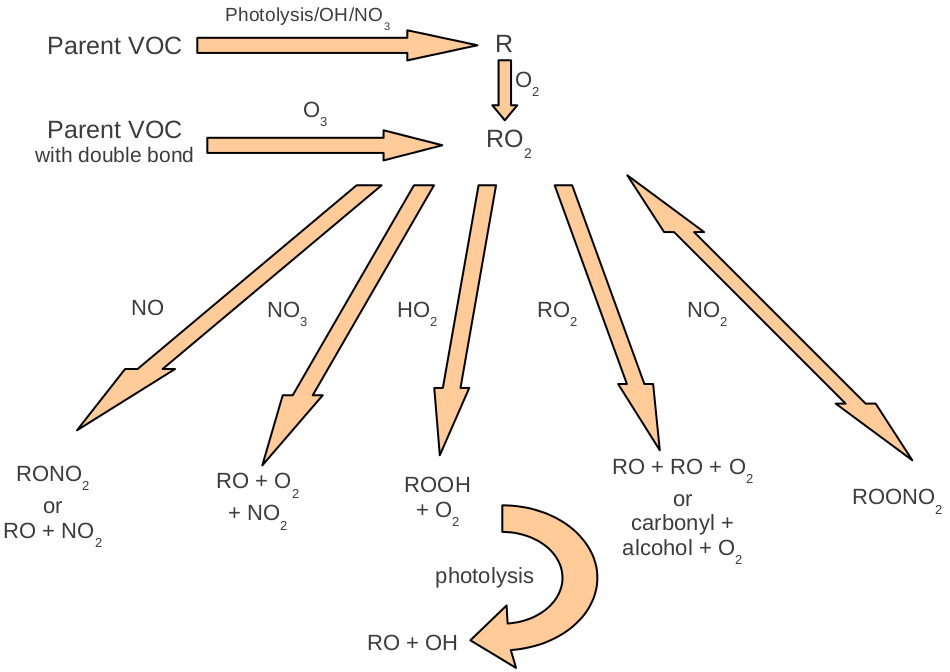
\includegraphics[height=100mm, width=120mm]{VOC_reaction_updated}
        \caption[what is this]{VOC reaction pathway}
        \label{f:VOC_reaction}
    \end{center}
\end{figure}

As noted earlier, the most common initiation reaction of a VOC is with the OH radical, and this forms an alkyl or substituted alkyl radical (R) depending on the parent VOC. 
The addition reaction with \ce{O2} then leads to the formation of alkyl peroxy radicals (\ce{RO2}). 
During the night-time, reaction with the \ce{NO3} radical is of importance and for VOCs containing a double bond, reaction with \ce{O3} also occurs. 
Photolysis is an important degradation initiator for carbonyl species, this is particularly important throughout the whole degradation mechanism of the VOC as carbonyl species, such as formaldehyde, are common reaction products. 
These initial reaction pathways all lead to the formation of \ce{RO2} radicals, as shown below.
\begin{reactionlist}
    \reactionitem{VOC + OH/\ce{NO3 / O3}/$h\upsilon$}{R}{new}{r:VOCinit}
    \reactionitem{R + \ce{O2}}{\ce{RO2}}{new}{r:R+O2}
\end{reactionlist} 
\ce{RO2} radicals can subsequently react with NO, \ce{NO2}, hydroperoxy (\ce{HO2}) radicals, \ce{NO3} radicals - mainly during night-time - and also with other alkyl peroxy radicals. 
The competition between these reactions determines the amount of net ozone production or loss from the parent VOC. 
\begin{reactionlist}
    \reactionitem{\ce{RO2 + NO + M}}{\ce{RONO2 + M}}{new}{r:RO2+NOa}
    \reactionitem{\ce{RO2 + NO}}{RO + \ce{NO2}}{new}{r:RO2+NOb}
    \reactionitemrev{\ce{RO2 + NO2 + M}}{\ce{ROONO2 + M}}{new}{r:RO2+NO2}
    \reactionitem{\ce{RO2 + HO2}}{ROOH + \ce{O2}}{new}{r:RO2+HO2}
    \reactionitem{\ce{RO2 + NO3}}{\ce{RO + NO2 + O2}}{new}{r:RO2+NO3}
    \reactionitem{\ce{RCH(OO)R$'$ + RCH(OO)R$'$}}{\ce{RCH(O)R$'$ + RCH(O)R$'$ + O2}}{new}{r:RCHOOR+RCHOORa} 
    \reactionitem{\ce{RCH(OO)R$'$ + RCH(OO)R$'$}}{\ce{RCH(OH)R$'$ + RC(O)R$'$ + O2}}{new}{r:RCHOOR+RCHOORb}
\end{reactionlist}
All pathways in Figure \ref{f:VOC_reaction} that lead to \ce{NO2} formation can result in \ce{O3} formation due to \reactionref{r:NO2photo} and \reactionref{r:O3form}. 
Reaction with the \ce{HO2} radical results in the formation of hydroperoxides (ROOH), which then photolyse to an alkoxy (RO) radical and the OH radical, this OH radical is then available to react with other VOCs. 
The carbonyl and alcohol products resulting from reaction with other \ce{RO2} radicals will follow a similar sequence of reactions and hence can also produce further \ce{O3}. 
Reaction with \ce{NO2} leads to the formation of alkyl peroxynitrates (\ce{ROONO2}), however this reaction product can be thermally unstable and may decompose quickly to the reactants, as mentioned in Section \ref{s:reservoir}.

The RO radical that results from many of the \ce{RO2} pathways undergoes further reactions, either by decomposition, isomerisation or reaction with \ce{O2}. 
The products that result from the reaction pathways depend on the parent VOC and this also determines the number of NO-to-\ce{NO2} conversions, eventually leading to \ce{O3} formation.

All VOCs and their degradation products will ultimately result in carbon dioxide (\ce{CO2}) and water vapour. 
The path that each VOC takes to reach its final products is dependent on the type of VOC, the radical concentration, the \ce{NO_x} concentration and other factors such as time of day and year. 
The detailed atmospheric chemistry of some simple VOCs is well-understood (for example, methane) however for more complex molecules, especially aromatic VOCs, there are a great number of uncertainties. 
These uncertainties can be related to kinetic data, photolysis rates, reaction branching ratios and in most cases the reaction products. 
Any uncertainties in reaction pathways and products of VOCs also leads to uncertainties in the ozone forming potential of the respective VOC \citep{Atkinson:2000}.

\subsection{\texorpdfstring{VOC and \ce{NO_x} Chemistry}{VOC and NOx Chemistry}} \label{s:VOC&NOx}
%balance of NOx & NMVOC for O3 production
As mentioned above, \ce{O3} chemistry is influenced by both VOC and \ce{NO_x} concentrations. 
Figure \ref{f:O3_isopleth} depicts the non-linear relationship between \ce{O3} concentration when considered as a function of VOC concentration (in ppmC, i.e. parts per million mass of a carbon unit of the VOC, \ce{CH_{2.5}}) and \ce{NO_x} concentration (in ppm, i.e. parts per million mass). 
\begin{figure}
	\begin{center}
		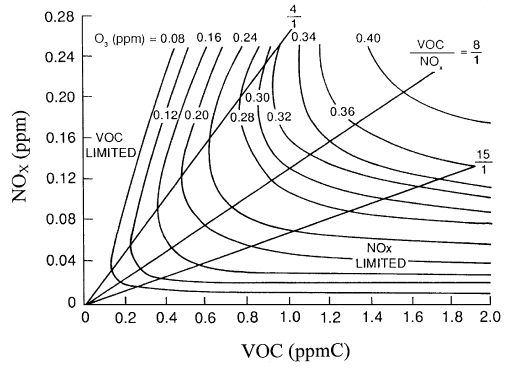
\includegraphics[height=90mm, width=85mm]{O3_isopleth_1.png}
		\caption{Ozone isopleth plots for various initial concentrations of \ce{NO_x} and a specified VOC mixture. Taken from \citep{Jenkin:2000}.}
		\label{f:O3_isopleth}
	\end{center}
\end{figure}

This relationship can be divided into distinct regimes: \textbf{\ce{NO_x}-sensitive}, \textbf{VOC-sensitive} and \textbf{VOC-and-\ce{NO_x}-sensitive}. 
The \ce{NO_x}-sensitive regime is the right-most part, the VOC-and-\ce{NO_x}-sensitive regime is the middle section and the VOC-sensitive regime is the left-most part of Figure \ref{f:O3_isopleth} and these correspond to high, middle and low VOC:\ce{NO_x} ratios, respectively. 
These different regimes arise from how the atmosphere removes \ce{NO_x} and radicals resulting from VOCs. 

In the \ce{NO_x}-sensitive regime, the concentration of \ce{NO_x} is low compared to that of radicals. 
Hence, peroxy radicals are removed by reaction with the OH radical such as 
\begin{reactionlist}
    \reactionitem{\ce{HO2 + OH}}{\ce{H2O + O2}}{new}{r:HO2+OH}
\end{reactionlist}
or by peroxy radical addition reactions.
\begin{reactionlist}
    \reactionitem{\ce{HO2 + HO2}}{\ce{H2O2}}{old}{r:HO2+HO2}
    \reactionitem{\ce{RO2 + HO2}}{\ce{ROOH + O2}}{old}{r:RO2+HO2}
\end{reactionlist}
This results in the NO concentration controlling the number of NO-to-\ce{NO2} conversions, rather than the concentration of peroxy radicals produced during VOC oxidation. 
An increase in NO conversion would thus promote \ce{O3} production due to an increase in \reactionref{r:NO2photo} and \reactionref{r:O3form} reactions. 
Increasing VOC concentrations would not increase \ce{O3} production as this only speeds up the formation of peroxy radicals and has no direct effect on the \ce{NO_x} concentration.

The VOC-sensitive regime corresponds to high \ce{NO_x} concentrations, hence radicals will tend to react with either NO or \ce{NO2}. 
Increasing \ce{NO_x} concentrations will not increase not increase \ce{O3} production as the \ce{NO_x} will react with the peroxy radicals resulting from VOC degradation. 
However, this increase in \ce{NO_x} increases the formation of nitric acid (\ce{HNO3}) by reaction with the OH radical \citep{Kleinman:1991, Kleinman:1994, Kirchner:2001}.
\begin{reactionlist}
    \reactionitem{\ce{OH + NO2}}{\ce{HNO3}}{new}{r:OH+NO2}
\end{reactionlist}
The competition of VOCs and \ce{NO_x} for reaction with the OH radical is at the heart of \ce{O3} production or destruction in the VOC-sensitive regime. 
Reaction of VOCs with the OH radical will produce more peroxy radicals, increasing \ce{O3} production whilst reaction of \ce{NO_x} increases \ce{HNO3} by \reactionref{r:OH+NO2} which reduces \ce{O3} production \citep{Kleinman:1991, Kleinman:1994, Kirchner:2001}.

The VOC-and-\ce{NO_x}-sensitive regime is characterised by \ce{O3} production being sensitive to both VOC and \ce{NO_x} concentrations. 
The turning point from a VOC-sensitive to a VOC-and-\ce{NO_x}-sensitive regime is when the maximum \ce{O3} production for a particular VOC concentration has been reached. 
The shift into a \ce{NO_x}-sensitive occurs when increases in VOC concentrations result in very little \ce{O3} production \citep{Kirchner:2001}. 
The non-linear relationship can be thought of as a titration process between the amount of radicals and the \ce{NO_x} present in the atmosphere.

This non-linear nature of the atmosphere must be taken into account when policymakers consider control strategies for \ce{O3} concentrations. 
The difficulty is exacerbated by the fact that regions can alternate between these regimes depending on the season, time of day etc. 

Moreover, an air parcel emitted in an urban area may also evolve as outlined in Figure \ref{f:air_parcel}, as it moves downwind. 
\begin{figure}
	\begin{center}
		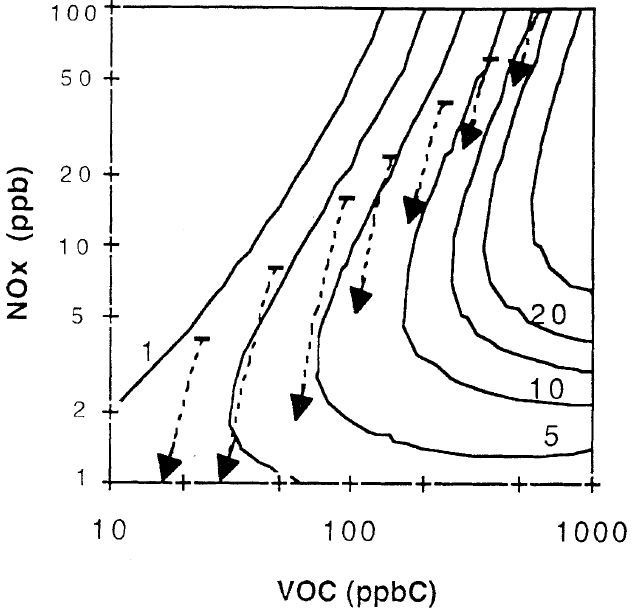
\includegraphics[height=80mm, width=75mm]{air_parcel.png}
		\caption{Air parcel evolution overlayed with ozone isopleth plots for various initial concentrations of \ce{NO_x} and VOCs. Taken from \citep{Sillman:1999}.}
		\label{f:air_parcel}
	\end{center}
\end{figure}
Once the air parcel has been emitted, it would typically fall into the VOC-sensitive regime but as the parcel ages it would move into the \ce{NO_x}-sensitive regime. 
Reducing VOC and \ce{NO_x} would reduce tropospheric \ce{O3}, whilst reducing VOC levels would only be effective during VOC-sensitive regimes and reducing \ce{NO_x} levels is only effective in \ce{NO_x}-sensitive regimes and can even increase \ce{O3} concentrations \citep{Sillman:1999}. 
This is due to the radical or \ce{NO_x} removal pathways that may or may not promote \ce{O3} production as discussed above.

\section{Ozone Production Potential}
%Ozone production potential of VOCs
The difficulty in applying uniform and successful emission control strategies due to the different regimes of the atmosphere has given rise to a more thorough investigation into the ozone production capabilities of different VOCs, also called the Ozone Production Potential (OPP) of the VOC in question. 
This potential can be calculated via modelling studies and has given rise to reactivity scales classifying the OPP of VOCs or classes of VOCs. 
The OPP of a VOC is dependent on the meteorological conditions, the reactivity of the VOC and the location of its emission. 
A wide range of such scales have been developed and are discussed below.

\subsection{MIR and MOIR Incremental Reactivity Scales} \label{s:MIR&MOIR}
%Carter incremental reactivity scales
\citep{Carter:1994} outlines three incremental reactivity scales, the Maximum Incremental Reactivity (MIR), Maximum Ozone Incremental Reactivty (MOIR) and Equal Benefit Incremental Reactivity (EBIR) scales. 
The incremental reactivity of a VOC is defined as the change in \ce{O3} concentration caused when adding a small amount of the VOC in question to the emissions. 
Incremental reactivities are typically investigated through modelling studies although they can also be determined by means of airshed studies. 

The VOC reactivity, mechanism pathways and the atmospheric regime into which it is emitted all influence the incremental reactivity value of the VOC. 
Hence, the total \ce{NO_x} available is extremely important, as this determines the atmospheric regime present. 
For example, in VOC-sensitive regimes, the VOCs will have larger incremental reactivities than in a \ce{NO_x}-sensitive regime.

The MIR scale is calculated by adjusting the \ce{NO_x} levels so that the largest incremental reactivity was achieved for the individual VOC. 
The MOIR scale differs from the MIR as it is calculated using \ce{NO_x} levels that give the maximum ozone concentration for the whole VOC mix.  
Whilst calculating the EBIR scale involves adjusting the \ce{NO_x} inputs so that the effect on \ce{O3} for a specific percentage change in VOC has the same effect of an equal percentange change in \ce{NO_x} \citep{Carter:1994}. 
The MOIR and EBIR scales are also shown in \citep{Carter:1994} to be practically equivalent when factoring in uncertainties during their calculation.

The MIR and MOIR scales are applicable to different regions due to their differences in \ce{NO_x} concentrations. 
The MIR scale is applicable to places that have high transport emissions such as Los Angeles, as this implies an increased amount of \ce{NO_x} in the atmosphere when compared with the amount of VOCs. 
In contrast, the MOIR scale is more relevant to areas that have higher VOC (biogenic or anthropogenic) emissions. 
However, both scales do not include transport or multi-day scenarios during their calculation and this may effect their applicability \citep{Capps:2010}.

\subsection{Photochemical Ozone Creation Potential}
%POCP
The Photochemical Ozone Creation Potential (POCP) was introduced in \citep{Derwent:1996} and was used to calculate ozone production under the conditions applicable to northwestern Europe. 
This is in contrast to the MIR and MOIR which are both applicable to the US, due to the \ce{NO_x} levels used for their calculations and that in Europe the transport of reactive species and multi-day photochemistry are more important. 
Hence, the POCP values are calculated over a five day period.

The POCP is calculated by increasing the amount of a VOC in a photochemical trajectory model and calculating the increase in \ce{O3} concentration. 
This is then expressed as a percentage using the ozone increase due to the same amount in mass of ethene as reference. 
The increased time period in the model runs to calculate the POCP values showed that almost all VOC increase their ozone formation potential over time. 
The exceptions to this are the highly reactive VOC as they are completely oxidised during the initial emission phase \citep{Derwent:1996}. 

The calculation of the POCP was further refined in \citep{Derwent:1998} by using a more detailed chemical mechanism in the atmospheric model than that used in \citep{Derwent:1996} and by also studying the influence of different \ce{NO_x} concentrations. 
The Master Chemical Mechanism (MCM) is used as this provides a lot of chemical detail in the reaction mechanisms of the VOCs. 

The general trend of the POCP values did not change when using the MCM, however the individual values themselves were affected.
The \ce{NO_x} inputs were also adjusted in order to mirror planned changes in \ce{NO_x} emission standards and to investigate the robustness of these planned policies if based on POCPs. 
Once again, the same general trend of the POCP values was noted, although there are some VOCs (e.g. 1,3-butadiene) whose reactivity changed drastically depending on the \ce{NO_x} conditions \citep{Derwent:1998}. 
This again demonstrates the importance of taking into consideration the different possible regimes in the atmosphere as described in Section \ref{s:VOC&NOx}.

%use of IR scales
The use of incremental reactivity scales has been used in regulatory control in some US cities \citep{Luecken:2008}, where the MIR has mainly been used for such purposes. 
Due to the assumptions made during the generation of the scale itself, such as the \ce{NO_x} levels, it is not straightforward to extend the use of an incremental reactivity scale to a larger geographical area.
Moreover, the incremental reactivity scales are typically calculated using a box-model which does not include such factors as meteorology and may not include effects of transported air masses that, as previously discussed, can all influence the amount of \ce{O3} produced. 

%disadvantages of incremental reactivity scales 
A VOC's direct or indirect impact on ozone production cannot be distinguished when using incremental reactivity scales. 
The direct impact is the incremental effect of both the extra VOC and the resulting oxidation intermediates. 
Whilst the indirect impact is the effect that these VOC increments have on the availability of radical species which in turn influences the ozone production from other compounds in the base VOC mixture \citep{Butler:2011}, as discussed in Section \ref{s:VOC&NOx}. 
Another disadvantage is that the reactivity scales do not include detailed chemical information on the oxidation reactions of the VOC and how this is related to the OPP, moreover some scales do not account for the temporal effects of ozone production.

\subsection{Tagged Ozone Production Potential} \label{s:TOPP}
%TOPP
This led to a new approach outlined in \citep{Butler:2011} that links the degradation products of VOCs by using a tagging approach, called the Tagged Ozone Production Potential (TOPP). 
The calculation of the TOPP is taken over multiple days and calculates the direct impact of a particular VOC on its total impact on the \ce{O_x} family, defined previously in Section \ref{s:reservoir}. 
The TOPP was calculated for NMVOCs listed in Table \ref{t:VOClist} and the atmospheric conditions related to Los Angeles and Beijing and gave similar results despite these two cities having different NMVOC profiles. 

The TOPP values also indicate two groups of NMVOCs, those that reach a maximum in the first day of the simulation followed by a decrease and those reaching a maximum TOPP after the first day. 
The first group includes many reactive NMVOCs such as alkenes and xylenes whilst the second group includes the slower reacting species such as alkanes and benzene. 
These groups can be determined as the time taken for a VOC to reach its maximum \ce{O3} production potential is dependent on the rate at which VOCs yield smaller peroxy radical oxidation fragments. 

\citep{Butler:2011} also compares the TOPP to the MIR, MOIR and POCP showing that the TOPP compares well with all three, although to differing degrees for different classes of NMVOCs in the cases of the MIR and MOIR. 
An added advantage of the tagging approach used for the TOPP calculations is that the reaction pathways of the VOC in question that contribute to \ce{O3} production can be determined. 
As in \citep{Butler:2011}, these reactions can be compared for different VOCs to determine the reactions that directly effect ozone production.

\section{Comparison of Chemical Mechanisms}
Given the different chemical mechanisms and their differing approaches towards simplifying the complexities of atmospheric chemistry, there have been many comparative studies to determine the differences between calculation results obtained when performing the same modelling study but altering the mechanism. 
In \citep{Dunker:1984} four mechanisms that were used in atmospheric modelling studies were compared by means of atmospheric simulations of box, trajectory and grid modelling studies and also against chamber study results. 
The comparison parameters were plotted \ce{O3}, \ce{NO2} and PAN isopleths as well as the time span required for the maximum one hour average \ce{O3}, \ce{NO2} and PAN concentrations to be reached. 
The largest differences between the mechanisms were found during the box model study whereas the other simulations correlated well. 
It is also highlighted that differences in chemistry can be masked by the effects of the meteorology and other parameters not included in a box model.

A study of the chemical mechanisms used mainly for European regional studies are compared in \citep{Gross:2003}. 
Here, a box model study with the three different mechanisms is used to generate the concentrations of \ce{O3}, NO, \ce{NO2}, \ce{OH} radical, \ce{HO2} radical and organic peroxy radicals \ce{RO2}. 
\ce{O3} isopleth plots are also generated by performing the study over a range of \ce{NO_x} and VOC concentrations. 
A common set of photolysis coefficients were used so that the results would mirror only differences in the chemistry, the study also accounted for both urban and rural conditions in separate model runs.

The results show that the greatest differences between these mechanisms are in the \ce{O3}, \ce{NO2} and \ce{RO2} radical concentrations. 
The differences in the \ce{O3} concentrations are linked to the discrepancies between the \ce{NO2} and \ce{RO2} concentrations as these are reactions that lead to \ce{O3} production or loss. 
This emphasises the importance of the treatment of organic peroxy radicals, which is typically one of the major areas of difference between chemical mechanisms. 
The rural study showed little difference in the comparison parameters whilst the urban study showed larger differences. 
This can be attributed to the complexity of the organic chemistry prevalent in urban areas. 
\citep{Gross:2003} recommends that many different urban scenarios be considered and that \ce{O3} isopleth plots giving the \ce{O3} concentration over a range of \ce{NO_x} and VOC values should be used for such mechanism comparison studies. 

\citep{Emmerson:2009} compares the gas-phase chemical mechanisms used in global models. 
Since the MCM contains more chemical details than the reduced schemes used in global models it is used as a reference to which these are compared. 
The comparison is performed by box model runs simulating a large number of scenarios that are characteristic of global situations - industrial, clean, cold and dry, hot and wet, biogenic and non-biogenic conditions. 
Moreover, a particular recorded event (where the data are taken from the summer 2003 TORCH campaign) is also simulated with all the models to determine how close the simulation results are to the actual recorded concentrations. 

The simulations were ran without heterogenous chemistry and all set to begin at midnight in order to investigate the effect of night-time chemistry, which would be affected most by not including heterogenous chemistry. 
The length of each simulation is five days as a compromise between very long and very short run times which can affect the chemistry in different ways. 
Long model runs would imply significant ageing of the air masses that would drive the chemistry and very short model runs would not test the chemistry pertaining to the degradation products at all, hence a compromise needs to be found. 
Separate model runs were also performed to determine differences in the inorganic chemistry, full chemistry and night-time chemistry.

The resulting concentrations of specific compounds were plotted and compared to verify where mechanistic differences arise. 
The little difference between inorganic chemistry regimes can be attributed to the differences between kinetic data supplied by IUPAC and JPL, whilst there are more differences between the full chemistry and night-time chemistry. 
The greatest differences in the organic chemistry is when biogenic compounds, such as isoprene, are considered and are present in larger concentrations. 
For the specific pollution event that was modelled, the greatest differences arise for the night-time chemistry and \ce{O3} concentrations.

Reactivity scales have also been used as comparison tool for chemical mechanisms, this was proposed as in a single number, they provide a lot chemical kinetic data. 
In \citep{Derwent:2010}, the MCM and SAPRC are compared by calculation of the POCP of 116 organic compounds from the major atmospheric classes within both mechanisms. 
A series of photochemical trajectory model runs simulating a single day were performed, many parameters other than the mechanisms were adjusted as incremental reactivities are not solely geophysical measures but rely on many other parameters.

The MCM and the SAPRC were chosen for this study as they are near-explicit mechanisms with the main difference being in how they treat the first generation products - the MCM continues in an explicit manner while the SAPRC uses aggregation techniques. 
In general, the POCP values correlate very well between the two mechanisms, with a small number of exceptions. 
These can be attributed to the lack of detailed understanding of the degradation reactions of these compounds. 
The good correlation of reactivities of the aromatic compounds merely indicates that both mechanisms treat aromatic compounds similarly rather than having a detailed knowledge of these degradation schemes.

A detailed look at the chemistry affecting different mechanisms used in air quality modelling is described in \citep{Stockwell:2012}, where a box modelling study is undertaken with near-explicit and aggregated chemical mechanisms. 
The model system used is the same as that used in \citep{Seefeld:1999} with only gas-phase chemistry and constant meteorological conditions.  
Different model runs were also undertaken with different temperatures in order to determine the temperature dependency of model results. 

The study highlights that the temperature dependence of gas phase reactions is uncertain for both organic and inorganic compounds. 
Also, night-time chemistry is a major source of uncertainty. 
Other knowledge gaps include the rate coefficients of the reactions of organic peroxy radicals as well as the products resulting from these reactions, the detailed degradation of both aromatic and biogenic compounds.  
